\documentclass{../Vorlage/mat}
\lstset{
	basicstyle=\small
}

\begin{document}
\maketitle{Sebastian Bliefert}{}{Nils Drebing}{}{Pascal Pieper}{}{08.02.2017}{5} \\

\section*{Aufgabe 1}
\begin{figure}[h!]
\centering
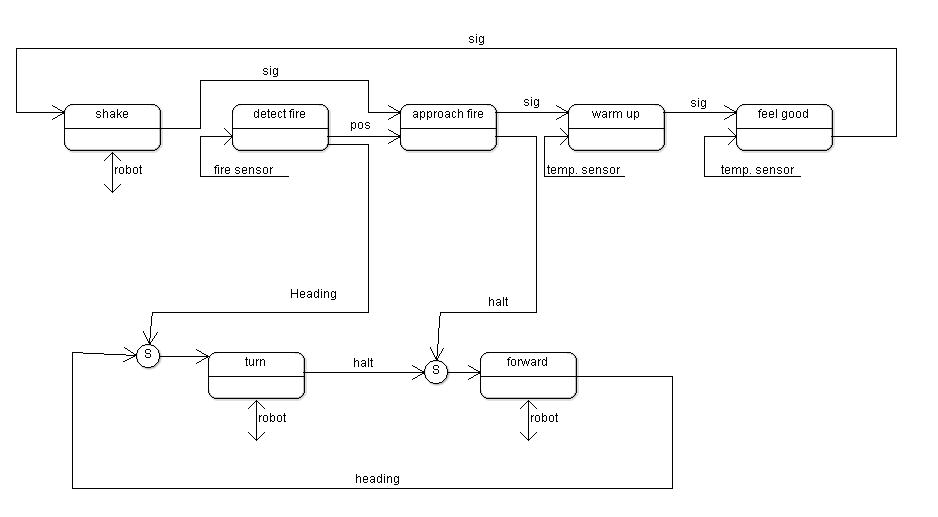
\includegraphics[width=\linewidth]{aufgabe1}
\label{fig:aufgabe1}
\caption{Subsumption-Architektur des Roboters}
\end{figure}

Bei der Erstellung des angegebenen Modells haben wir uns folgendes gedacht:\\
\textbf{Ebene 1:}\\
\begin{itemize}
	\item \texttt{forward} sendet durchgehend eine konstante Richtung nämlich geradeaus. Ansonsten fährt es mit einer konstanten Geschwindigkeit geradeaus solange es kein halt Signal bekommt.
	\item \texttt{turn} bekommt Informationen über die gewünschte Bewegungsrichtung und von einem Hindernissensor beliebiger Art. Mit diesen Informationen dreht \texttt{turn} den Roboter in die richtige Richtung. Es kann den Roboter ebenfalls zum stoppen bringen indem es ein halt Signal an \texttt{forward schickt.}
\end{itemize}
\textbf{Ebene 2:}
\begin{itemize}
	\item \texttt{shake} sendet das Schüttelsignal direkt an die Aktuatoren. Weiterhin wird ein start Signal an \texttt{approach fire} gesendet.
	\item \texttt{detect fire} entdeckt mit Hilfe eines geeigneten Sensors ein Feuer und gibt dessen relative Position an \texttt{approach fire} weiter. Dies tut es durchgehend.
	\item \texttt{approach fire} erhält von \texttt{detect fire} durchgehend die relative Position des nächsten Feuers. Sobald ein Startsignal von \texttt{shake} eingegangen ist überschreibt es den heading Eingang von \texttt{turn} um den Roboter in die nähe des Feuers zu bringen. Sobald er in der Nähe ist wird ein Signal an \texttt{warm up} weitergegeben und das Modul schaltet sich ab, bis zum nächsten Startsignal.
	\item \texttt{warm up} erhält Temperaturdaten von einem geeigneten Sensor und schickt so lange ein halt Signal an \texttt{forward} bis der Roboter wieder genügend aufgewärmt ist. Dann sendet es ein Startsignal an \texttt{feel good} und schaltet sich ab.
	\item \texttt{feel good} erhält durchgehend Temperaturdaten von einem geeigneten Sensor und sendet ein Startsignal an \texttt{shake} sobald die Temperatur zu gering ist.
\end{itemize}


\section*{Aufgabe 2}
\subsection*{a)}
Die Implementierung ist aus dem Sourcecode der \textit{behaviour.py} zu entnehmen.

Obstacle Avoidance überprüft die Sensoren, ob die inneren Sensoren unter 25 cm und die äußeren Sensoren unter 15 cm melden. Wenn sie das tun, wird entweder zurück oder vorwärts leicht links oder rechts, je nach Seite, ausgewichen.

Der Autonomous Drive überprüft, ob seine Ausrichtung zu dem nächsten Wegpunkt innerhalb einer Toleranzgrenze liegt. Wenn ja, fährt er geradeaus. Wenn nicht, dreht er sich, bis er ihn trifft. Weiterhin merkt er, wenn sein Rotationspunkt (nicht der Mittelpunkt) innerhalb einer Toleranzentfernung liegt. Sobald das erreicht ist, aktualisiert er seinen  Wegfindungsalgorithmus (Weg), und fährt weiter. Wenn der letzte Wegpunkt erreicht wird (Mit der Mitte, und nicht mit dem Rotationspunkt), wird angehalten.
\newpage
\subsection*{b)}
\begin{figure}[!htbp]
\centering
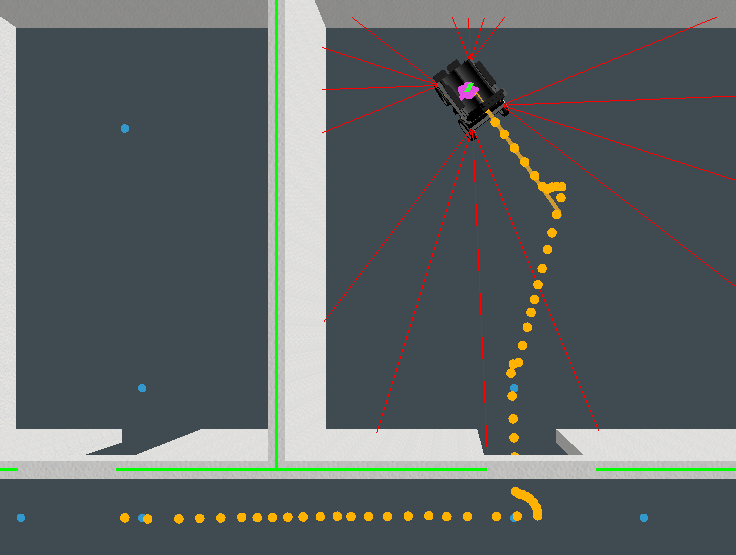
\includegraphics[scale=0.3]{forwards}
\label{fig:aufgabe2b1}
\caption{Weg der Rollstuhls beim Vorwärtsfahren (Punkte in Orange sind tatsächlicher Weg)}
\end{figure}

\begin{figure}[!htbp]
\centering
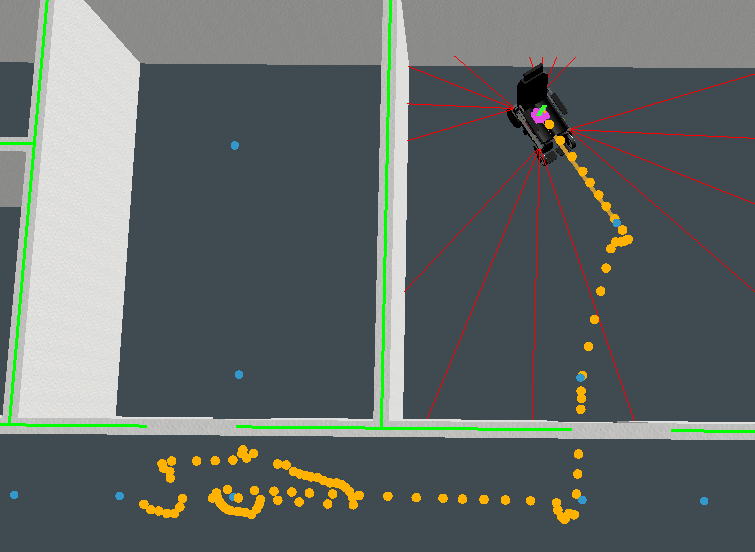
\includegraphics[scale=0.3]{backwards}
\label{fig:aufgabe2b2}
\caption{Weg der Rollstuhls beim Rückwärtsfahren (Punkte in Orange sind tatsächlicher Weg)}

\end{figure}


\subsection*{c)}
Das Umschalten der Modi wird durch eine Änderung der \textit{backwards}-Variable in der \textit{behaviour.py} möglich.

Aus Sicht der Implementierung ist die Steuerung für das Vorwärtsfahren lediglich invertiert und somit kein großer Programmieraufwand. Allerdings fährt der Rollstuhl zunächst einmal rückwärts im Kreis, bis er anschließend dem Weg folgt.\\
Physikalisch betrachtet verhält sich der Rollstuhl bei der Rotation während des Rückwärtsfahrens insgesamt stabiler als bei einer Vorwärtsbewegung. 

\end{document}
